\documentclass[conference]{IEEEtran}
\pagestyle{plain}
\hyphenation{op-tical net-works semi-conduc-tor}

\usepackage{todonotes}
\usepackage[tight,footnotesize]{subfigure}

\usepackage{hyperref}
\hypersetup{
	breaklinks,
    pdfpagemode={UseOutlines},
    bookmarksopen,
    pdfstartview={FitH},
    colorlinks,
    linkcolor={blue},
    citecolor={red},
    urlcolor={blue}
}


\begin{document}
\title{
Distributed Security Risks and Opportunities \\
in the %\\
W3C Web of Things
}
\author{
  \IEEEauthorblockN{Michael McCool}
  \IEEEauthorblockA{Intel Corporation\\
                    michael.mccool@intel.com}
\and
  \IEEEauthorblockN{Elena Reshetova}
  \IEEEauthorblockA{Intel Corporation\\
                    elena.reshetova@intel.com}
}

\IEEEoverridecommandlockouts
\makeatletter\def\@IEEEpubidpullup{9\baselineskip}\makeatother
\IEEEpubid{\parbox{\columnwidth}{Permission to freely reproduce all or part
    of this paper for noncommercial purposes is granted provided that
    copies bear this notice and the full citation on the first
    page. Reproduction for commercial purposes is strictly prohibited
    without the prior written consent of the Internet Society, the
    first-named author (for reproduction of an entire paper only), and
    the author's employer if the paper was prepared within the scope
    of employment.  \\
    NDSS '18, 18-21 February 2018, San Diego, CA, USA\\
    Copyright 2018 Internet Society, ISBN 1-1891562-49-5\\
    http://dx.doi.org/10.14722/ndss.2018.23xxx
}
\hspace{\columnsep}\makebox[\columnwidth]{}}
\maketitle

\begin{abstract}
The W3C Web of Things (WoT) WG has been developing an interoperability standard for IoT devices that includes as
its main deliverable a ``Thing Description'': a standardized representation the metadata of an 
IoT device, including in particular its network interface, but also allowing for semantic annotation.
Relative to other approaches to IoT, such metadata has at least four major implications.
First, it allows for system-wide vulnerability analysis, 
which can be both a risk and an opportunity.
Second, metadata can enable end-to-end security in multistandards networks,
avoiding exposing data within bridges otherwise needed for connecting standards pairwise.
Third, metadata supports service and device discovery,
which raises the question of how to limit discovery to authorized agents.
Fourth, metadata can enable distributed security mechanisms for access control and micropayments.
To the extent that metadata access can be decentralized, decentralized mechanisms for security can
be supported, although several practical issues currently make this difficult to fully support.

\end{abstract}

% Introduction: state main goals and context of paper
\section{Introduction}
The economic impact of the IoT will be strongly dependent on how well devices from 
different manufacturers can interoperate.
Very often interoperability is taken for granted when estimating the business
benefit of IoT. 
However, if devices do \emph{not} interoperate,
a recent study \cite{McK2015a} concluded that 40\% to 60\% of the 
benefit of IoT will be unattainable,
due to the inability to address use cases that cannot be satisfied by a single manufacturer.

Unfortunately full interoperability is hard to achieve.
There are currently many competing IoT standards under development,
each of which is attempting to address this problem.
Most of these standards are prescriptive.
In a prescriptive standard,
devices are validated against specific requirements.
Typically the goal is that devices validated against particular standard will interoperate with
other devices also validated against that standard.
In addition, it is possible to bridge multiple standards so that
devices validated against one standard can communicate with
devices using another standard by translating communication protocols and payloads.
Of course if one standard comes to dominate bridging will be unnecessary.
However, so far such unification seems to be elusive and may be impossible due to
divergent requirements in different but overlapping IoT subdomains.

%Unfortunately the prescriptive approach has some weaknesses.
In addition to the issue of the interoperability for modern prescriptive IoT standards, there are always going to be devices that follow older standards or specifications.
There are decades-old devices in particular domains, such as building and factory
automation, that are just now being connected to the IoT.
These devices often represent major investments and cannot be economically replaced with newer,
standards-conforming devices.
This is the ``brownfield'' problem.
Moreover new devices are being deployed today that have not been validated
against any particular IoT standard,
even if they use other standards such as JSON and HTTP.

As an alternative to the prescriptive approach,
the W3C Web of Things (WoT) Working Group has been developing a \emph{descriptive} 
approach to IoT interoperability.
In the descriptive approach,
metadata is provided that describes how to communicate with each particular device.
The metadata itself is standardized but flexible enough to describe a wide variety of
IoT network interfaces.
With this approach,
devices can but do not have to be prevalidated against 
a particular standard before being deployed.
They can be described after the fact,
and do not need any modification to be
used as part of a Web of Things system.
This solves the brownfield problem and allows
older devices as well as devices satisfying different IoT 
standards to be integrated into a unified system.  

This approach has both risks and opportunities from a security point of view.

Most obviously, IoT devices, even those conforming to a prescriptive IoT standard,
may vary widely in their support for security.
Therefore a Web of Things system
needs to manage different levels of trust for different devices.
Devices from different ecosystems or manufacturers may also take different approaches to
security and may use different security mechanisms. 
This may cause integration challenges, even if the necessary
information is provided in the metadata.

Beyond this basic concern,
the availability of pervasive metadata raises several other issues
from a security perspective.
In this paper we discuss five major issues:
% NOTE: want to use {description} here but it seems to be broken...
\begin{enumerate}
\item \textbf{Local Links:}
End-point IoT devices can be deployed in many ways: starting from a closed, only locally accessible,
network behind a proxy or a firewall and ending with a globally addressed network. 
As a result the metadata provided by IoT devices should allow for expression of
different ways (links) how devices can be reached on a given network
and a way to securely update this information when the deployment setup changes. 
\item \textbf{Vulnerability Analysis:}
Providing information about what devices can do makes it easier to 
automatically scan for devices with vulnerabilities.
An attacker may also use this information to plan attacks that take advantage of 
vulnerabilities in multiple devices. 
However, for the system manager, scanning can also be an opportunity 
to identify devices whose vulnerabilities need to be mitigated.
\item \textbf{Endpoint Adaptation:}
Metadata enables end-to-end security in networks of IoT devices using multiple standards.
If metadata is used to push payload adaptation to endpoints then 
communication payloads can be encrypted end-to-end.  
This contrasts with systems that use local bridging to connect devices from multiple IoT standards.
Local bridges require opening (and usually re-encrypting) data in potentially-vulnerable gateways.
\item \textbf{Secure Discovery:}
Information about how to use a service, 
and ideally even its existence, should not
be disclosed to agents without the authorization to use it.
The WoT approach allows powerful semantic searches to be used for discovery.
How can this capability be made available while still securing the metadata?
\item \textbf{Enabling Distributed Security:}
Metadata may be provided to enable specific security mechanisms,
as well as features with security implications such as payment or scripting.
What mechanisms are needed and what data needs to be provided?
Also, depending on how the metadata is made available, it may or may not be 
possible to support decentralized approaches to security.
\end{enumerate}

The next few sections first introduce the W3C Web of Things draft standard,
focusing on the Thing Description metadata format.  
Then the high-level WoT Threat model will be introduced,
which includes a model of stakeholders, assets, attackers,
and threats, as well as a typical WoT deployment scenario.
Once this context has been established, we will discuss in detail the above
five issues.



% Explain background (in this case, WoT) 
\section{Web of Things}
% Nowadays the amount of different IoT devices around us is 
% constantly increasing in all areas starting from smart home and ending up with industry automation. 
% All these devices target different use cases,
% have different underlying implementations and connected using different communication protocols.
% In this light 
The Web of Things (WoT)~\cite{Wot2017arch} aims to provide interoperability between IoT devices.
It does this by defining a metadata format,
the WoT \emph{Thing Description}, that can describe 
a wide range of IoT network interfaces.
A Thing Description can describe the network interfaces of existing devices
or can be produced and consumed by devices running a WoT runtime supporting a WoT scripting
API that normalizes interactions with other devices with a common abstraction layer.


\subsection{Architecture}
%\textsf{Web of Things architecture \cite{Wot2017arch}, Thing Description \cite{Wot2017td} and
%scripting API \cite{Wot2017script}.}

The WoT architecture\cite{Wot2017arch} defines three basic entities that can be organized in a various set of configurations and topologies based on a concrete deployment scenario:

\begin{itemize}
	\item A \textbf{WoT Thing} represents a physical or virtual IoT device and exposes a network-facing API for interaction.
	Each WoT Thing has an associated Thing Description (TD)\cite{Wot2017td} that is a set of metadata describing relevant information about the Thing, such as general information, available interactions, communication and security mechanisms.
	A typical example of a WoT Thing might be a garage door controller, providing a number of actions that can be performed on a garage door, i.e. \textit{open}, \textit{close}, etc.
	\item A \textbf{WoT Client} is an entity that wants to perform an action on a WoT Thing.
	It is able to consume a TD provided by a WoT Thing and issue actions on exposed WoT interfaces.
	For example a WoT Client might be a browser or an application on a user's smartphone that allows user to operate the garage door controller. 
	\item A \textbf{WoT Servient} can be viewed as a combination of above two, i.e. an entity that is both providing one or more WoT things and also at the same time is able to operate as WoT Client on other WoT things.
	An example of a WoT servient is a home gateway device that acts as a WoT client towards home appliance WoT things (such as different lights and sensors) and also exposes some higher level virtual devices (such as all the lights in the living room) in form of the WoT Things available for user's smartphone WoT Client.
\end{itemize}

Internally a typical architecture of a WoT Servient is shown in Figure~\ref{fig-fservient}. 
In addition to a Thing Description (TD) it also has WoT Binding Templates that can be used to instantiate a TD for a particular IoT protocol binding, such as OCF, COAP etc. 
The last remaining part is WoT Scripting API, which is an optional component that allows implementing the Thing logic in a higher-level programming language and browser-like environment (such as JavaScript). 

\begin{figure}[!t]
\centering
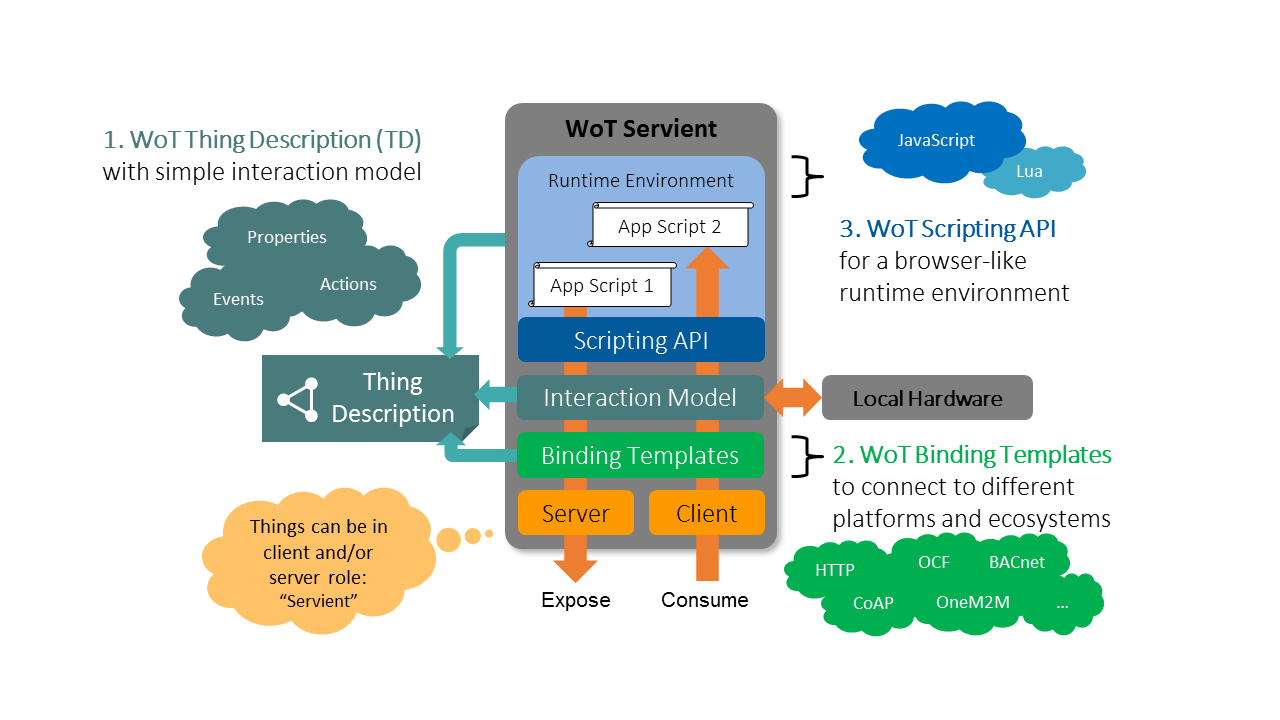
\includegraphics[width=4in]{figures/wot-servient.png}
\caption{WoT Servient architecture}
\label{fig-fservient}
\end{figure}




\subsection{Threat Model}
%\textsf{A basic intro to to the WoT threat model \cite{Wot2017sec}.}

Due to the large diversity of devices, use cases, deployment scenarios and various requirements for WoT Things, it is impossible to define a single WoT threat model that would fit every case.
Instead we have created an overall WoT threat model~\cite{Wot2017sec} that can be adjusted by OEMs or other WoT system users or providers based on their concrete security requirements.

%The WoT threat model defines the following key WoT Assets that are important from security point of view:	\textit{Thing Description}, \textit{Thing User Data} (any user data transferred via WoT network, such as video streams, sensor data etc.), \textit{Thing Provider Data} (WoT application scripts and their configuration data), \textit{WoT Basic Security Metadata} (all provisioned security medatada), \textit{WoT Controlled Environment} (physical environment that can be affected by WoT Things), \textit{WoT Thing and Infrastructure Resources} (resources of devices providing WoT Things and overall WoT network) and \textit{WoT Behavior Metrics} (all indirectly transmitted information).
%Some of these assets might be absent and/or have different trust model (i.e who should have a legitimate access and to what extent) depending on deployment scenario. 

The threat model defines security-relevant WoT assets and a set of WoT threats on these assets that can be in- or out-of-scope based deployment scenario, security objectives, risks etc.
For example, in a smart home scenario involving WoT things that record audio/video information a privacy aspect is very important and therefore this type of data has high confidentiality requirements.
On another hand, in industry automation scenario involving WoT things that control some safety-critical infrastructure, confidentiality might not be the highest priority, but availability of the WoT Thing and Infrastructure Resources and protection of WoT Controlled Environment is of topmost importance.

Being a distributed system brings an additional complexity angle to the WoT Threat Model and the choice of relevant security mitigations.
One cannot anymore rely on standard communication infrastructure and protocols (like HTTPS) to provide an end-to-end security between all communicating parties, and instead WoT needs to enable supporting different set of security mechanisms (potentially nested or interdependent) that can be combined into single end-to-end security solution.  
  
 



\subsection{Typical Deployment Scenario}
%\textsf{Usage scenarios.}

Figure~\ref{fig-wot-scenario} presents a typical WoT deployment scenario. 
A WoT Thing device together with a WoT Servient are placed inside 
the local network behind a forwarding proxy. 
A WoT Client that is located outside of this boundary wants to 
perform operations on the WoT Thing and WoT Servient.
The available operations are given in corresponding Thing Descriptions.
There are various ways Thing Descriptions provided by WoT Things
could be made available to WoT Clients.
In this case, the Thing Descriptions are 
uploaded by the WoT Thing and WoT Servient to a Thing Directory.
A Thing Directory is a service which can be accessed by Clients
to search for WoT Things it can communicate with.
In order to do this the WoT Client first needs to issue a 
discovery query to the Thing Directory.
Thing Directories can support semantic search capabilities, allowing
Things to be discovered based on semantic annotations. 
Access to the search capabilities of a Thing Directory should
only be provided to authorized clients, as with any web service.
Upon obtaining a Thing Description, 
the WoT Client needs to make sure it has all the necessary credentials
to authenticate to the forwarding proxy 
(if secure authentication on proxy is enabled), 
the WoT Servient and in some cases even to the end WoT Thing.
All required information about these potentially different 
credentials should be provided in the obtained Thing Description.  

\begin{figure*}[!t]
\centering
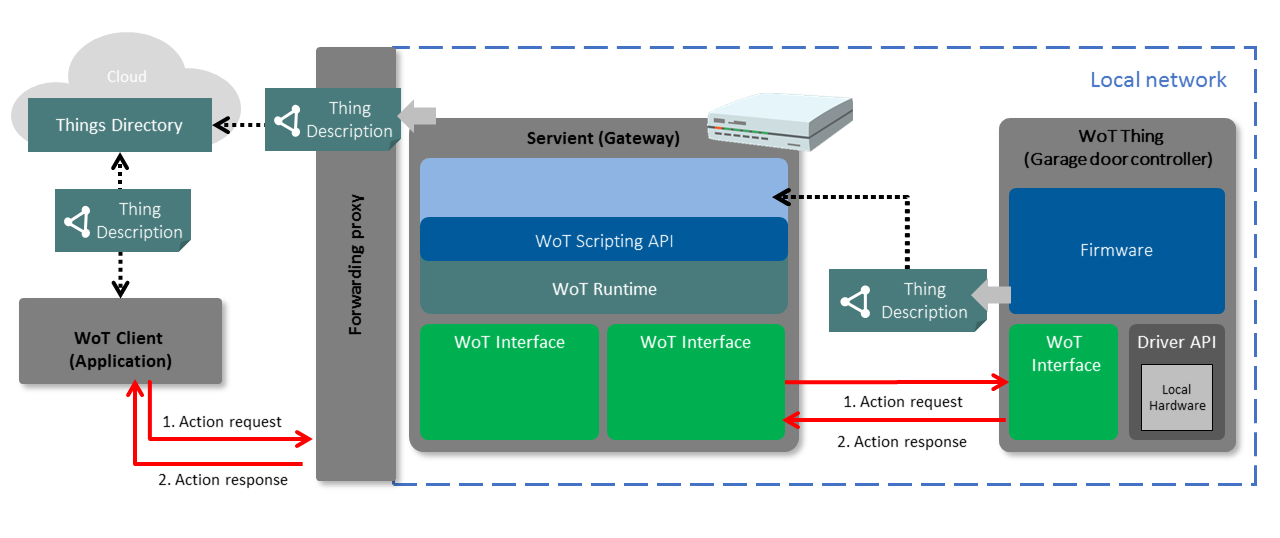
\includegraphics[width=6in]{figures/wot-scenario.png}
\caption{Typical WoT deployment scenario}
\label{fig-wot-scenario}
\end{figure*}



% Best practices in IoT that are *common* to WoT... and that we will NOT focus on
% We want to explain in particular how WoT is different
\section{Related Work}
% Some relevant prior work: 
% State-of-the-Art and Challenges for the Internet of Things Security \cite{Garcia2017a}.
% The Industrial Internet of Things Security Framework \cite{Iic2016sf}.
% IoT Security Foundation Best Practices Guidelines \cite{Iotsf2017a}.
The WoT approach applies to a wide diversity of IoT devices and use cases.
It has to take be able to support best practices in IoT security which
are however still rapidly evolving.
Recently some attempts have been made to define
best practices for IoT security.
The IETF Thing-to-Thing Research group has a RFP under development,
\emph{State-of-the-Art and Challenges for the Internet of Things 
Security}\cite{Garcia2017a}, which includes a threat model similar to 
what we have defined for the WoT.  However, it does not consider the 
importance of protecting access to descriptive metadata.
The Industrial Internet of Things has published a comprehensive
\emph{Security Framework}\cite{Iic2016sf}.
This is useful, but focuses on industrial use cases.
The IoT Security Foundation has published
a \textit{Best Practices Guidelines}\cite{Iotsf2017a}
document as well.
All three documents consider various additional factors we do
not have time to go into here, such as trust management over the 
lifecycle of the device.

In addition there are many papers(~\cite{Iot2020},~\cite{Xu2014},~\cite{Fernandes2017} and others)  that attempt to describe 
the current IoT security challenges and provide suggestions for the future work in the area.





% What are some specific interesting problems/solutions that WoT brings?
\section{Risks and Opportunities}
\label{sec-risks-opportunities}

\subsection{Local Links}
Practical pitfalls.  HTTPS not working locally.  Local links vs global links in Thing Directories.


\subsection{Vulnerability Scanning}
\textsf{Vulnerability scanning using metadata.}


\subsection{Endpoint Adaptation}
% \textsf{End-to-end secure adaptation by pushing payload transformation to endpoints.}
In a typical multistandard IoT system,
bridges may be needed to connect devices
conforming to different standards.
For example,
to connect to an AllJoyn device from a controller
designed to connect to OCF devices, an OCF-to-AllJoyn bridge
may be needed to translate both the protocol and the payload.
In general, multiple bridges could be involved: the
apparent AllJoyn device could in fact be a oneM2M device
being made available over yet another bridge.

Unfortunately bridges introduce a potential security vulnerability.
If the bridge devices can be compromised,
they have full access to the
data being carried to and from the device can can stage a 
variety of attacks: 
modifying or deleting data,
injecting false data and events,
or privacy invasion.

The WoT enables a way around this problem using end-to-end encryption.
Basically, rather than adapting payloads in a point-to-point fashion,
adaptation should take place at one of the endpoints, ideally the
one with greater capability.  The endpoint doing the adaptation should
look at the metadata for the target endpoint, adapt its payload for that
target, and then use end-to-end encrypted communication.
It may still be necessary to use bridges in between to adapt protocols
(for example, bridging from HTTPS on the internet to CoAPS over a local
network) but the payloads can remain encrypted.



\subsection{Secure Discovery}
\textsf{Secure semantic searches.  How do we ensure only the data permitted for a user is used in a search?}
Some possibly relevant papers: \cite{Thura2005,Xia2014}.


\subsection{Enabling Distributed Security}
\textsf{Metadata for distributed security and payment mechanisms.}



\section{Conclusion}
\textsf{Conclusions.  What are the main points?}


\section*{Acknowledgment}
\textsf{Thank you, thank you, all!}


\bibliographystyle{IEEEtranS}
\bibliography{refs}
\end{document}


